%-------------------------------------------------------------------------------
%-------------------------------------------------------------------------------
\begin{frame}\begin{center}
	\LARGE\textbf{Truncation and Censoring}
\end{center}\end{frame}
%-------------------------------------------------------------------------------
%-------------------------------------------------------------------------------
\begin{frame}
	\textbf{Setup}\\
	\begin{align*}
	\begin{pmatrix}
	Z \\
	I
	\end{pmatrix}  \sim \mathcal{N} \left(
	\begin{pmatrix}
	0 \\
	0
	\end{pmatrix} , \begin{pmatrix}
	1.0  &  \rho \\
	\rho &  1.0
	\end{pmatrix} \right)
	\end{align*}

\end{frame}
%-------------------------------------------------------------------------------
%-------------------------------------------------------------------------------
\begin{frame}
\begin{figure}[htp]\centering
\caption{Density of truncated standard Normal distribution}
\scalebox{0.35}{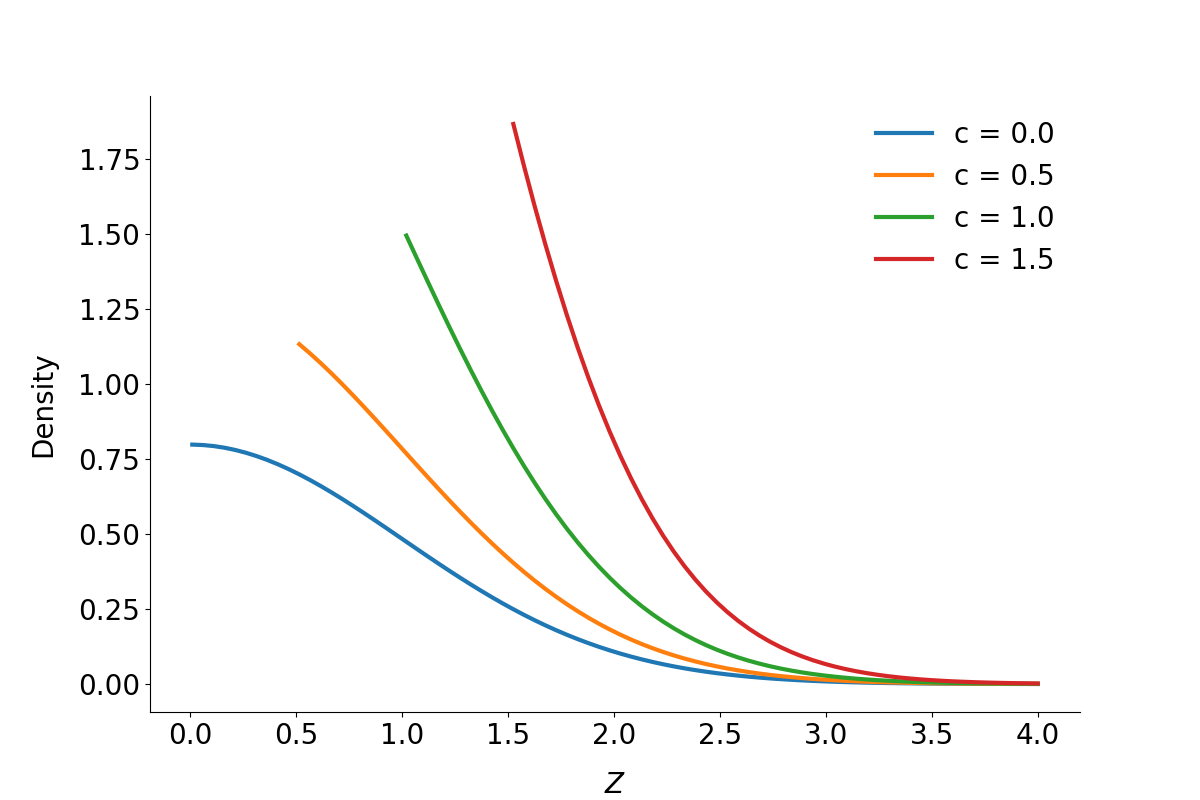
\includegraphics{fig-truncated-normal-density}}
\end{figure}
\end{frame}

\begin{frame}
\begin{figure}[htp]\centering
\caption{Expectation of truncated standard Normal distribution}
\scalebox{0.35}{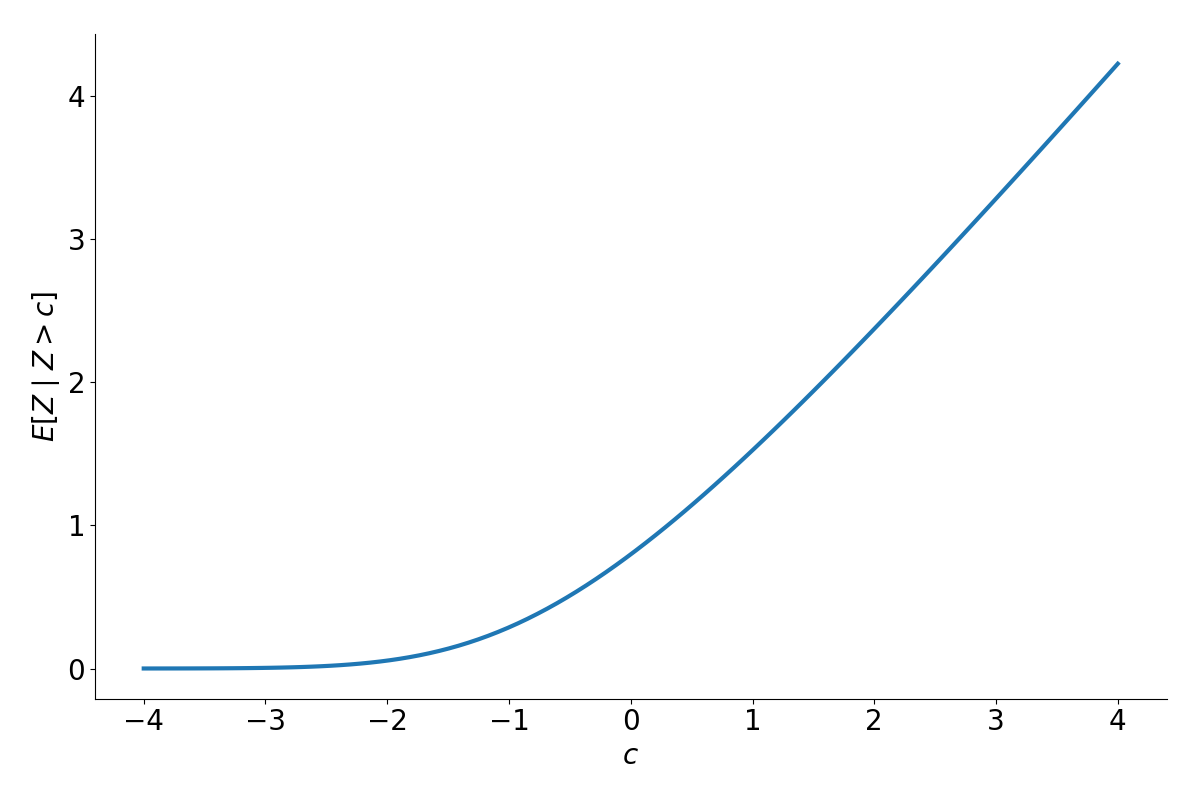
\includegraphics{fig-truncated-normal-expectation}}
\end{figure}
\end{frame}

\begin{frame}
\begin{figure}[htp]\centering
\caption{Variance of truncated standard Normal distribution}
\scalebox{0.35}{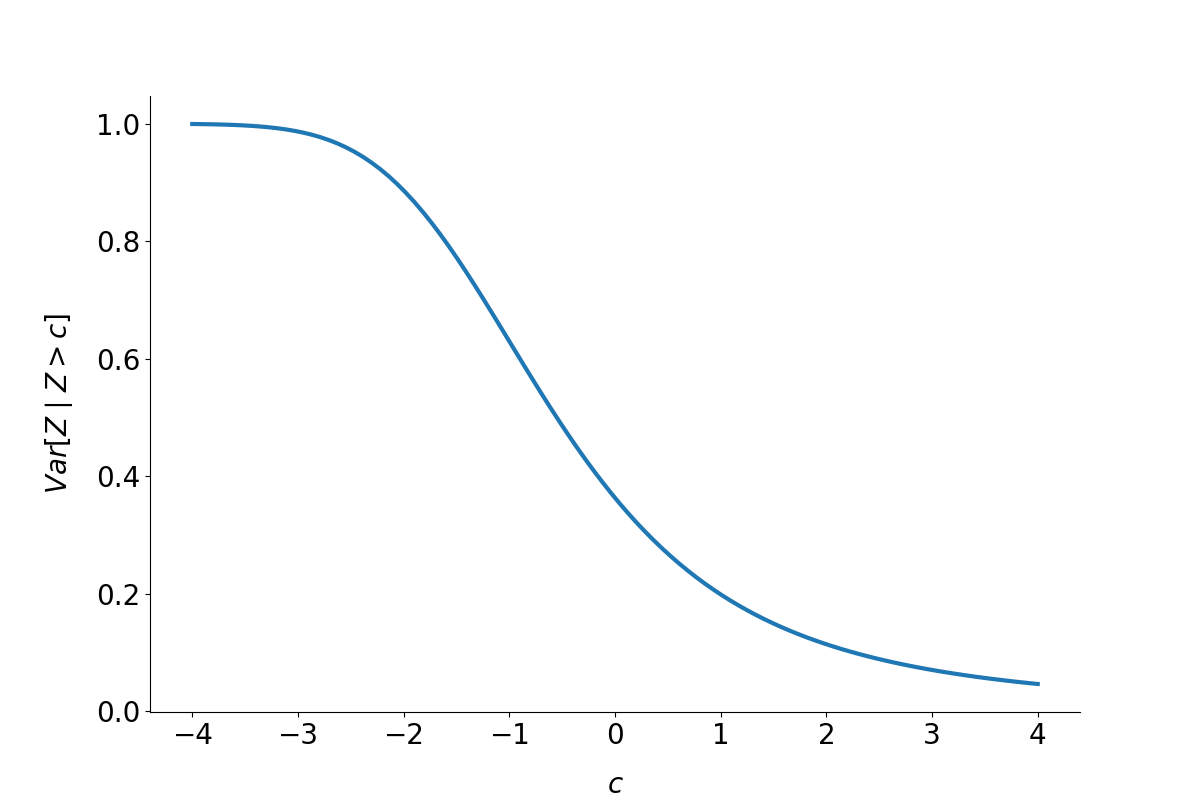
\includegraphics{fig-truncated-normal-variance}}
\end{figure}
\end{frame}
%---------------------------------------------------------------------------------------------------
%---------------------------------------------------------------------------------------------------
\begin{frame}
\begin{figure}[htp]\centering
\caption{Density of censored standard Normal distribution}
\scalebox{0.35}{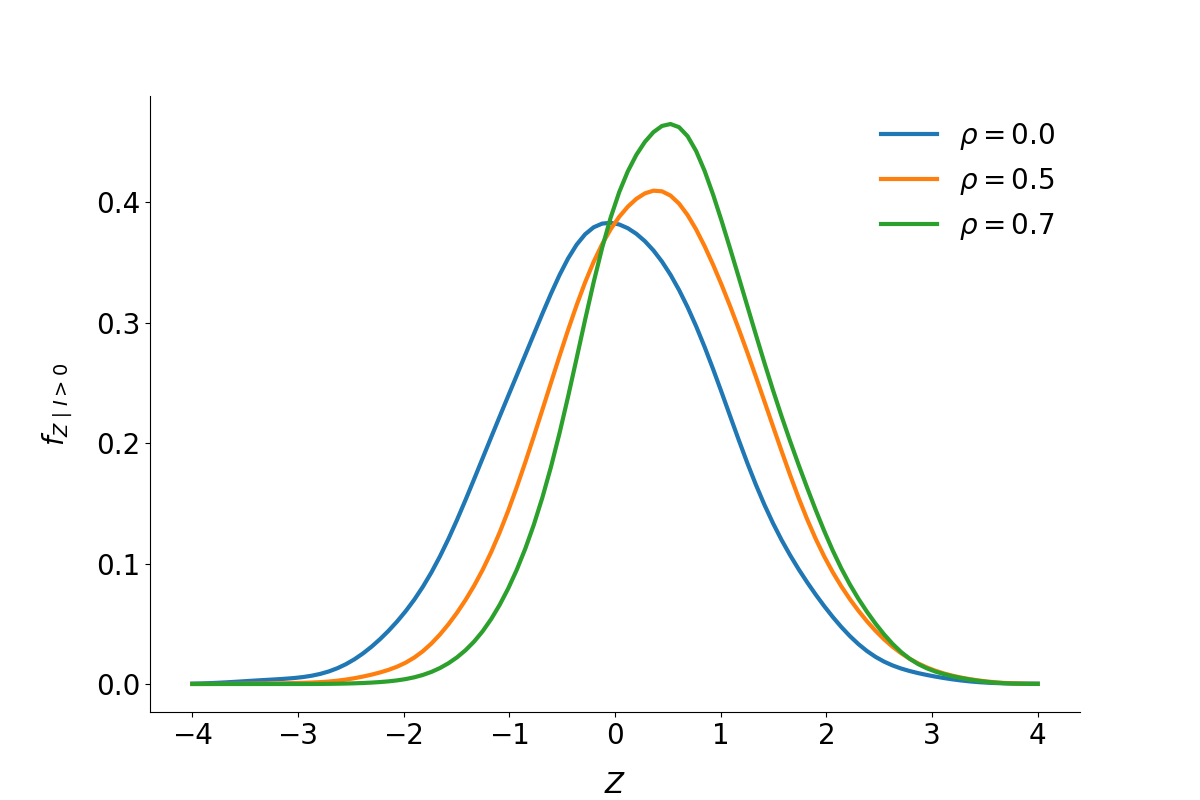
\includegraphics{fig-censored-normal-density}}
\end{figure}
\end{frame}
%-------------------------------------------------------------------------------
%-------------------------------------------------------------------------------
\begin{frame}\begin{center}
	\LARGE\textbf{Sorting and selection}
\end{center}\end{frame}
%---------------------------------------------------------------------------------------------------
%---------------------------------------------------------------------------------------------------
\begin{frame}
	\textbf{Wage Equations}
	\begin{align*}
	\ln W_1 & = \ln \pi_1 + \mu_1 + U_1 \\
	\ln W_2 & = \ln \pi_2 + \mu_2 + U_2, \\
	\end{align*}
	where $U_i = \ln S_i - \mu_i$.
\end{frame}
%-------------------------------------------------------------------------------
%-------------------------------------------------------------------------------
\begin{frame}
	\textbf{Some notation}
	\begin{align*}
	\sigma^* & = \sigma_{U_1 - U_0} \\
			& = \sqrt{(\sigma_{11} - \sigma_{12}) +  (\sigma_{22} - \sigma_{12})}\\
			& \\
	c^*_1 & = \left(\ln(\pi_1 / \pi_2) + \mu_1 - \mu_2\right)  / \sigma^* \\
	        & \\
 		L & = U_1 - U_0
	\end{align*}
\end{frame}
%-------------------------------------------------------------------------------
%-------------------------------------------------------------------------------
\begin{frame}
	\textbf{Selection bias}
	\begin{align*}
	E[\ln W_1 \mid \ln W_1 > \ln W_2] & = \ln \pi_1 + \mu_1 + E[U_1 \mid L > -c^*_1] \\
									  & = \hdots + E[U_1 \mid U_1 - U_0 > -c^*_1]
	\end{align*}

	\begin{itemize}
	\item What about identification at infinity arguments?
	\end{itemize}

\end{frame}
%-------------------------------------------------------------------------------
%-------------------------------------------------------------------------------
\begin{frame}
	\textbf{Sorting}
	\begin{align*}
	E[\ln S_1 \mid \ln W_1 > \ln W_2] & = \mu_1 + \frac{\sigma_{11} - \sigma_{12}}{\sigma^*} \lambda(-c_1) \\
	E[\ln S_2 \mid \ln W_2 > \ln W_1] & = \mu_2 + \frac{\sigma_{22} - \sigma_{12}}{\sigma^*} \lambda(-c_2)
	\end{align*}
	We know the following:
	\begin{align*}
	\sigma^* & = (\sigma_{11} - \sigma_{12}) +  (\sigma_{22} - \sigma_{12}) > 0 \\
	\lambda, \lambda^\prime &> 0
	\end{align*}
	\begin{itemize}\setlength\itemsep{1em}
		\item There must be positive selection into one of the occupations and there can be positive selection into both.
	\end{itemize}
\end{frame}
%-------------------------------------------------------------------------------
%-------------------------------------------------------------------------------
\begin{frame}
	\begin{figure}[htp]\centering
		\caption{Marginal Distributions of Skills}\label{Marginal Distributions of Skills}\scalebox{0.35}{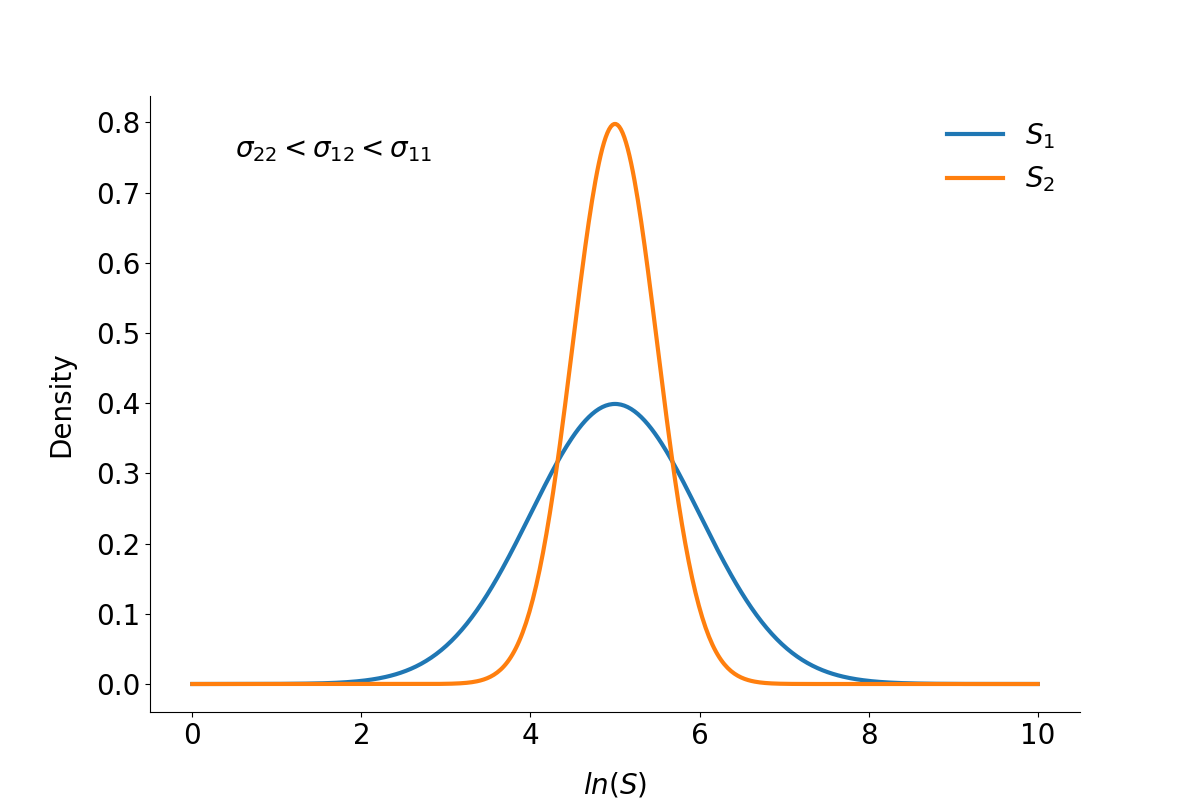
\includegraphics{fig-distribution-skills-latent-marginal-two}}
	\end{figure}
\end{frame}
%-------------------------------------------------------------------------------
%-------------------------------------------------------------------------------
\begin{frame}
	\textbf{What do we know?}\medskip
	\begin{itemize}\setlength\itemsep{1em}
	\item There is positive selection in Sector 1 as $\sigma_{11} > \sigma_{12}$.
	\item There is negative selection in Sector 2 as $\sigma_{22} < \sigma_{12}$.
	\end{itemize}
\end{frame}
%-------------------------------------------------------------------------------
%-------------------------------------------------------------------------------
\begin{frame}
	We gain further insights into the effect of self-selection on the distribution of earnings for workers in sector 1 by looking at the  distribution of $\ln S_1$  conditional on $\ln S_2$.
	\begin{align*}
	\ln S_1 \mid \ln S_2 \sim \N (\mu, \sigma),
	\end{align*}
	where
	\begin{align*}
	\mu = \mu_1 + \frac{\sigma_{12}}{\sigma_{22}} \Bigg(\ln S_2 - \mu_2\Bigg) \quad\text{and}\quad
	\sigma = \sigma_{11} \left(1 - \left(\frac{\sigma_{12}}{\sigma_1 \sigma_2}\right)^2\right)
	\end{align*}
\end{frame}
%---------------------------------------------------------------------------------------------------
%---------------------------------------------------------------------------------------------------
\begin{frame}
	\begin{center}
		\LARGE\textbf{Heckman Productions}
	\end{center}
\end{frame}
%---------------------------------------------------------------------------------------------------
%---------------------------------------------------------------------------------------------------
{
   \setbeamercolor{background canvas}{bg=}
	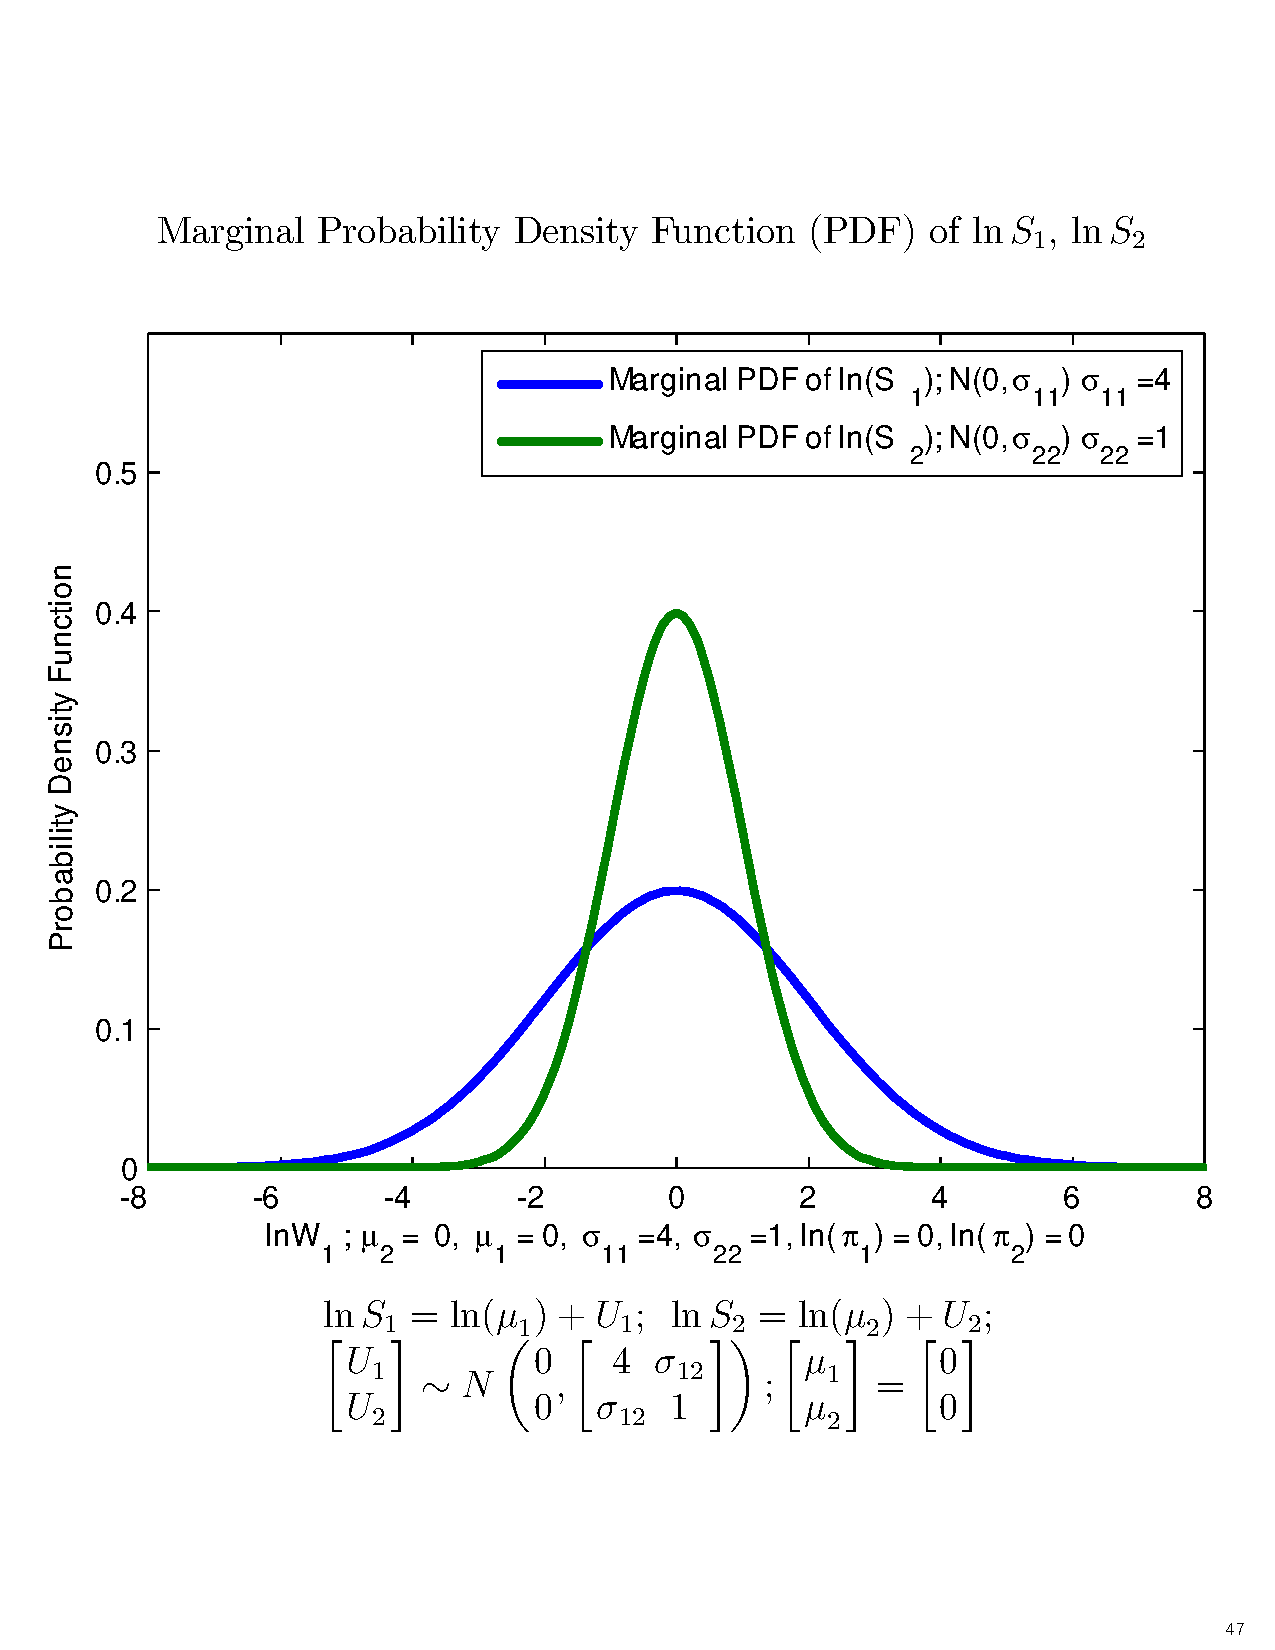
\includepdf[pages=1-100]{movie.pdf}
}
%---------------------------------------------------------------------------------------------------
%---------------------------------------------------------------------------------------------------
\begin{frame}\begin{center}
	\LARGE\textit{Change in skill prices}
\end{center}\end{frame}
%---------------------------------------------------------------------------------------------------
%---------------------------------------------------------------------------------------------------
\begin{frame}
\begin{align*}
E[\ln S_1 \mid \ln W_1 > \ln W_2] & = \mu_1 + \frac{\sigma_{11} - \sigma_{12}}{\sigma^*} \lambda(-c_1) > \mu_1\\
								  & \rightarrow \text{positive selection} \\
								  & \\
E[\ln S_2 \mid \ln W_2 > \ln W_1] & = \mu_2 + \frac{\sigma_{22} - \sigma_{12}}{\sigma^*} \lambda(-c_2) < \mu_2 \\
& \rightarrow \text{negative selection}
\end{align*}
, where $c_i = \ln(\pi_i / \pi_j) + \mu_i - \mu_j$



\end{frame}

\begin{frame}

How does the skill composition react to a change in prices?

\begin{align*}
\frac{E[\ln S_1 \mid \ln W_1 > \ln W_2]}{\partial \ln \pi_1 } & < 0 \\
&\\
\frac{E[\ln S_2 \mid \ln W_2 > \ln W_1]}{\partial \ln \pi_2 } & > 0
\end{align*}

\begin{itemize}
\item What are the underlying economics?
\end{itemize}

\end{frame}
